\documentclass[a4paper, 11pt, twocolumn]{article}

\usepackage[a4paper, total={6.24in, 8.5in}]{geometry}
\usepackage[utf8]{inputenc}
\usepackage{graphicx}
\usepackage{verbatim}
\usepackage{float}
\usepackage{array}
\usepackage{xfrac}
\usepackage{mathpazo}
\usepackage{amsmath}
\usepackage{bm}
\usepackage{multirow}
\usepackage{makecell}
\usepackage{multicol}
\usepackage{sectsty,textcase}
\usepackage{wrapfig,lipsum,booktabs}
\usepackage{enumitem}
\usepackage{hyperref}

\bibliographystyle{plain}
% \renewcommand{\thesubsection}{\alph{subsection})}
\renewcommand{\thesection}{\arabic{section}}
%\renewcommand{\baselinestretch}{1.02}

%\setlength\parindent{0pt}
\setlength{\columnsep}{15pt}
\newcommand{\myparagraph}[1]{\paragraph{#1}\mbox{}\\}

\title{FYS-STK3155/4155 Applied Data Analysis and Machine Learning - Project 2: Classification and Regression }

\author{Lotsberg, Bernhard Nornes \\ Nguyen, Anh-Nguyet Lise \and \url{https://github.com/liseanh/FYS-STK4155-project2/}}
\date{October - November 2019}
\begin{document}
\twocolumn[
  \begin{@twocolumnfalse}
    \maketitle
    \begin{abstract}
      blip blop opnion wrong
    \end{abstract}
  \end{@twocolumnfalse}
]

\section{Introduction}
Classification in statistical analysis is a useful tool, e.g. for predicting outcomes of various situations or classifying and sorting large amounts of data. 

The aim of this project is  to study classification and regression problems through our own implementation of logistic regression and a multilayer perceptron (MLP) in Python. This particular data set has been used in a prior research paper by Yeh, I. C. and Che-hui Lien about data mining techniques \cite{origarticle}, and can be downloaded from the \href{https://archive.ics.uci.edu/ml/datasets/default+of+credit+card+clients}{UCI Machine Learning Repository} \cite{UCI}.
We will use these methods to classify data of credit card clients' default payment from a Taiwanese bank. Additionally, we will use the MLP to solve a regression problem on Franke's function and compare the result from a prior project where we used standard least squares to solve the regression problem \cite{regpaper}.  


\section{Theory}

\subsection{Logistic Regression (LR)}
For classification.

Sigmoid function
\begin{equation}
p(t) = \frac{1}{1 + e^{-t}} =\frac{e^t}{e^t+1}
\end{equation}

\subsection{Artificial Neural Networks (ANN)}
An artificial neural network (ANN) is a computational model consisting of interconnected nodes. The interconnected nodes aim to emulate a simplified biological neural network in a brain  and neuronal firing, and are therefore also commonly referred to as neurons.  The node performs a weighted sum of its inputs that is subsequently passed through a mathematical function to determine its output. This mathematical function is called an activation function. The output value of the node can be adjusted for different purposes by choosing an appropriate activation function. 

There is a wide variety of different neural networks. Commonly, they consist of layers of nodes separated into the input layer and output layer, and may also contain one or more in-between layers called hidden layers. One such ANN is the multilayer perceptron (MLP), which is what we will be using in this project for both classification and regression. 
\subsubsection{Multilayer perceptron (MLP)}
The multilayer perceptron is a feed-forward neural network (FFNN), which means that the information flows forward only, starting from the input layer and to the output layer. Additionally, if each of the nodes in a layer is connected to all of the nodes in the succeeding layer, the network is fully connected. The inputs of the node are the weighted outputs of the nodes from the preceding layer, in addition to a bias term that can control whether or not the neuron fires if all the inputs are zero \cite{ML_algo}. 

The activation of the $j$th neuron of layer $l$ is defined as 
\begin{equation}
z_j^l = \sum_{i=1}^{M_{l-1}} w_{ij}^la_j^{l-1} + b_j^l,
\end{equation}
where $b_j^l$ and $w_{ij}^l$ are the biases and weights at layer $l$, and $a_j^l=f(z_j^l) $.

To calculate the optimal biases and weights for the problem, we initialize the gradients of the cost function $\mathcal{C}$ with respect to the  weights $W$ and biases $b$ at the output  layer $l=L$ 	and the output error $\delta_L$ as
\begin{flalign}
&\frac{\partial  \mathcal{C}}{\partial w^L_{jk}} = \delta^L_j a_k^{L-1}, \\
&\frac{\partial  \mathcal{C}}{\partial b^L_j} = \delta^L_j,\\
&\delta_j^L= f'(z_j^L)\frac{\partial \mathcal{C}}{\partial a_j^L},
\end{flalign}
before propagating backwards through the hidden layers using the general equations
\begin{flalign}
&\frac{\partial  \mathcal{C}}{\partial w^l_{jk}} = \delta^l_j a_k^{l-1}, \\
&\frac{\partial  \mathcal{C}}{\partial b^l_j} = \delta^l_j,\\
&\delta_j^l= \sum_k \delta_k^{l+1}w_{kj}^{l+1}f'(z_j^l).
\end{flalign}
Looking at these equations, it is clear that the chosen cost function $\mathcal{C}$ and the activation function $f(z)$ should be differentiable. 

The biases can be initialized to zero, but we have chosen an initial value of 0.01 to ensure that all of the neurons have some initial output. Initializing the weights to zero, however, will result in all neurons outputting the same value. Instead, the  weights are initialized with values drawn from a uniform distribution such that $w_{kj}\in (-1/\sqrt{n}, \ 1/\sqrt{n})$, where $n$ is the amount of nodes in the input layer,  to ensure uniform learning \cite{ML_algo}. 

\subsection{Stochastic Gradient Descent (SGD)}
It is clear that in order to find the best possible fit, we need to optimize the cost function $\mathcal{C}$ by finding its minimum. A common method to achieve this is the gradient descent (GD) method, in which the parameters $\theta$ are iteratively adjusted in the direction of the largest negative value of the gradient for a given number of iterations or until it reaches a given tolerance. Mathematically, this is expressed as
\begin{equation}
\theta_{i+1} = \theta_i -\eta \nabla \mathcal{C}(\theta_i),
\end{equation}
where $\eta$ is the learning rate, which is a hyperparameter that controls the step length and by extension the convergence time. For smaller values of $\eta$, the method will take longer to converge or might not converge at all within a desired time frame. For larger values of $\eta$, the method might be unstable or pass the minimum altogether and diverge. The parameter $\theta$ is $\beta$ in the LR case, and the weights $W$ and biases $b$ in the MLP case.  
However, calculating the gradient on the entire data set can be computationally expensive and inefficient for large amounts of data. Additionally, there is a high possibility of a local minimum being misinterpreted as a global minimum by the algorithm. 
To alleviate these problems, we can use stochastic gradient descent (SGD) with minibatches.  A minibatch is a subset of the data, on which we can perform GD. By using stochasticity to perform gradient descent on randomly chosen minibatches of size $M$, we have a more efficient way to approximate the gradient of the total data set as it might not need to use the entire set. Additionally, the stochasticity reduces the possibility of getting stuck in a local minimum.

\section{Data}
\subsection{Classification - Credit card client data}
For the classification part of this project,  we are using credit card payment data from a Taiwanese bank downloaded from the \href{https://archive.ics.uci.edu/ml/datasets/default+of+credit+card+clients}{UCI Machine Learning Repository}. The response variable is a binary variable of default payment with Yes = 1, No = 0.  The original data set consists of 30 000 observations, with X amount of observations with default payments. There are 23 explanatory variables, cited from the original paper they are described as \cite{origarticle}:
\begin{itemize}[leftmargin=5mm, itemsep=0pt,  parsep=1pt]
 \item X1: Amount of the given credit (NT dollar): it includes both the individual consumer credit and his/her family (supplementary) credit.
\item X2: Gender (1 = male; 2 = female).
\item X3: Education (1 = graduate school; 2 = university; 3 = high school; 4 = others).
\item X4: Marital status (1 = married; 2 = single; 3 = others).
\item X5: Age (year).
\item X6 - X11: History of past payment. We tracked the past monthly payment records (from April to September, 2005) as follows: X6 = the repayment status in September, 2005; X7 = the repayment status in August, 2005; . . .;X11 = the repayment status in April, 2005. The measurement scale for the repayment status is: -1 = pay duly; 1 = payment delay for one month; 2 = payment delay for two months; . . .; 8 = payment delay for eight months; 9 = payment delay for nine months and above.
\item X12-X17: Amount of bill statement (NT dollar). X12 = amount of bill statement in September, 2005; X13 = amount of bill statement in August, 2005; . . .; X17 = amount of bill statement in April, 2005.
\item X18-X23: Amount of previous payment (NT dollar). X18 = amount paid in September, 2005; X19 = amount paid in August, 2005; . . .; X23 = amount paid in April, 2005.
\end{itemize}

\subsection{Regression - Franke's function}
For the regression part part of this project we will be performing regression analysis on Franke's function $g(x,y)$ with added Gaussian noise $\bm{\varepsilon} \sim N(0,\  \sigma^2) $. Franke's function is given by 
\begin{align}
g(x,y) &= \frac{3}{4}\exp{\left(-\frac{(9x-2)^2}{4}   - \frac{(9y-2)^2}{4}\right)} \nonumber\\
 &+\frac{3}{4}\exp{\left(-\frac{(9x+1)^2}{49}- \frac{(9y+1)}{10}\right)} \nonumber\\
 &+\frac{1}{2}\exp{\left(-\frac{(9x-7)^2}{4} - \frac{(9y-3)^2}{4}\right)} \nonumber\\
 &-\frac{1}{5}\exp{\left(-(9x-4)^2 - (9y-7)^2\right) }  \label{eq:Franke}
\end{align} and is defined on $x,\ y \in [0,1]$. The data we are fitting is given by 
$$G(\bm{x}, \bm{y}) = g(\bm{x}, \bm{y}) + \bm{\varepsilon},$$
where $\bm{x},\ \bm{y}$ are vectors of uniformly spaced values from 0 and 1 of size $(1\times n_x)$ and $(1\times n_y)$ respectively. To directly compare with our previous project, \textit{Project 1: Regression analysis and resampling methods} \cite{regpaper}, we choose to generate and analyze the following data sets: 
\begin{itemize}[leftmargin=7mm, itemsep=5pt,  parsep=1pt, topsep=3pt]
\item 400 total data points of $G(\bm{x}, \bm{y}) $ with $\sigma=1$, $n_x=n_y=20$.
\item 400 total data points of $G(\bm{x}, \bm{y}) $ with $\sigma=0.1$, $n_x=n_y=20$ .
\item 40 000 total data points with $\sigma=0.1$, $n_x=n_y=200$ .
\end{itemize}  

\section{Model evaluation}
\subsection{Regression}
To evaluate the performance of our regression model, we consider the $R^2$ score, given by 
\begin{equation}
    R^2(\bm{y}, \bm{\hat{y}}) = 1 - \frac{\sum_{i=0}^{n - 1} (y_i - \hat{y}_i)^2}{\sum_{i=0}^{n - 1} (y_i - \bar{y})^2},
    \label{eq:R2}
\end{equation}
where $\bm{y}$ is the given data, $\bm{\hat{y}}$ is the model and ${\bar{y}}$ is the mean value of $\bm{y}$.
\subsection{Classification}
To evaluate the performance of our classification model, we consider the accuracy score, given by 
\begin{equation}
\label{eq:accuracy}
\text{accuracy}=\frac{\sum_{i=1}^nI(t_i=y_i)}{n},
\end{equation}
where $t_i$ is the target, $y_i$ is the model output, $n$ is the number of samples and $I$ is the indicator function, 
\[
I = \begin{cases} 
1, & t_i = y_i\\
0, & t_i \neq y_i
\end{cases} .
\]

\section{Method}




\section{Results}

\begin{figure}[H]
	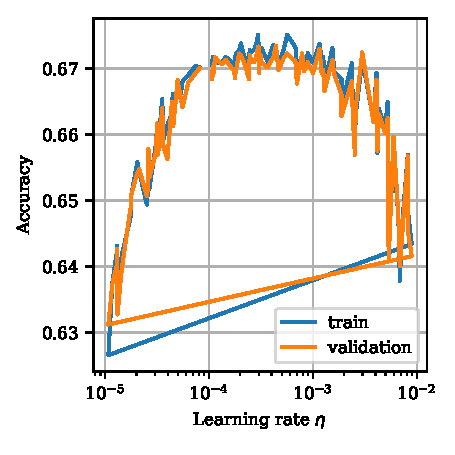
\includegraphics[scale=1]{figures/logreg_learning_rate_accuracy.pdf}
	\caption{Accuracy score of validation set of the credit card data using the logistic regression classifier. The values of the shrinkage parameter $\lambda$ were chosen using randomized search.}
\end{figure}

\begin{figure}[H]
	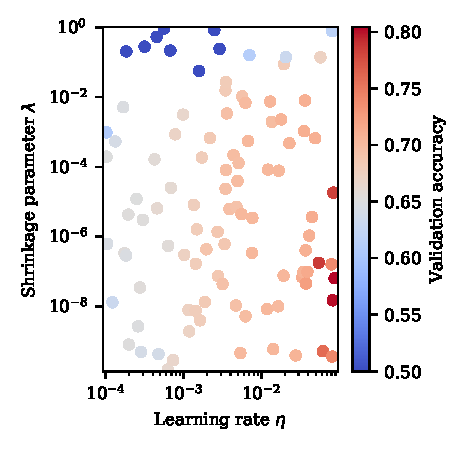
\includegraphics[scale=1]{figures/nn_learning_rate_lambda_accuracy_credit.pdf}
	\caption{Accuracy score of validation set of the credit card data using the multilayer perceptron classifier. The values of the shrinkage parameter $\lambda$ and the learning rate $\eta$ were chosen using randomized search.}
\end{figure}


\begin{figure}[H]
	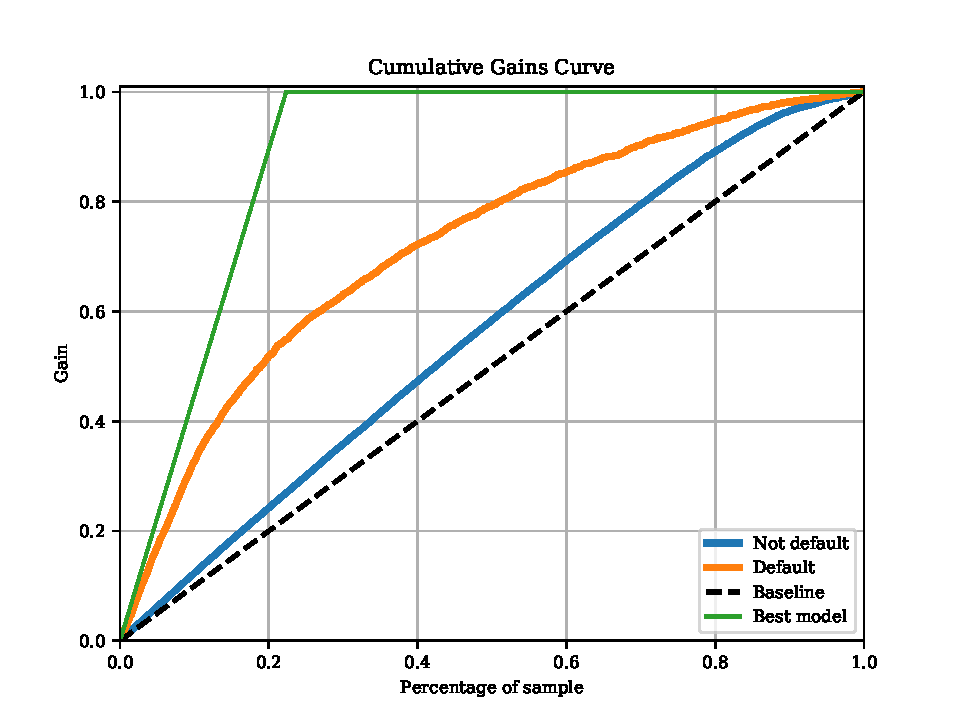
\includegraphics[scale=1]{figures/cumulative_gain_NN.pdf}
	\caption{idk yet}
\end{figure}

\begin{figure}[H]
	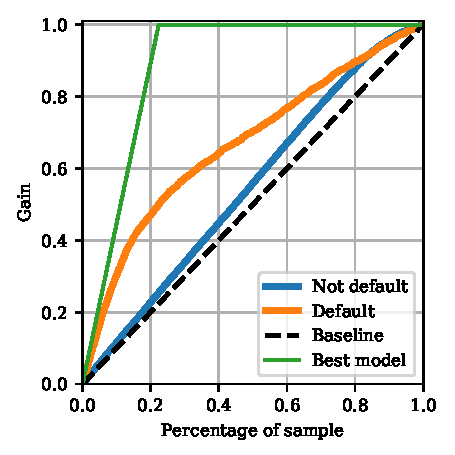
\includegraphics[scale=1]{figures/cumulative_gain_logreg.pdf}
	\caption{idk yet}
\end{figure}


\begin{figure}
	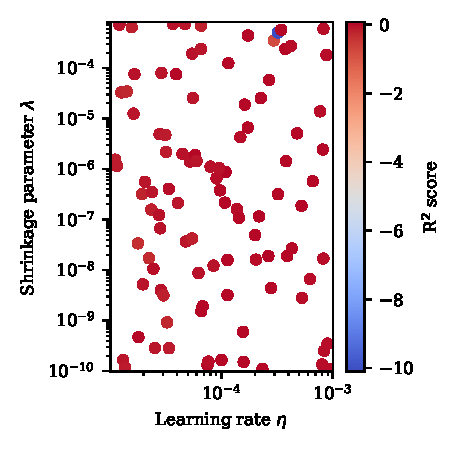
\includegraphics[scale=1]{{figures/nn_learning_rate_lambda_r2_franke_20_20_1.0}.pdf}
	\caption{$R^2$ score of validation set of the Franke function data set with 400 total points $n_x=n_y=20,\ \sigma=1.0$ using the multilayer perceptron regressor. The values of the shrinkage parameter $\lambda$ and the learning rate $\eta$ were chosen using randomized grid search.}
\end{figure}


\begin{figure}
	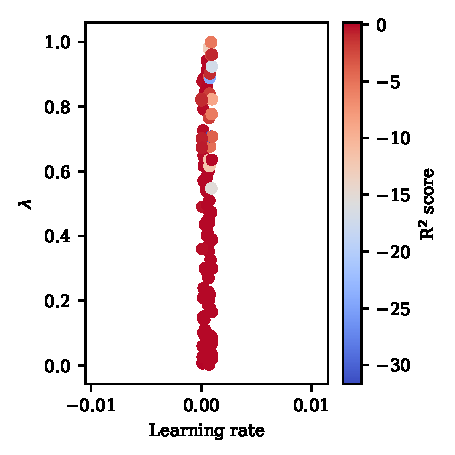
\includegraphics[scale=1]{{figures/nn_learning_rate_lambda_r2_franke_20_20_0.1}.pdf}
	\caption{$R^2$ score of validation set of the Franke function data set with 400 total points, $n_x=n_y=20,\ \sigma=0.1 $ using the multilayer perceptron regressor. The values of the shrinkage parameter $\lambda$ and the learning rate $\eta$ were chosen using randomized grid search.}
\end{figure}


\begin{figure}
	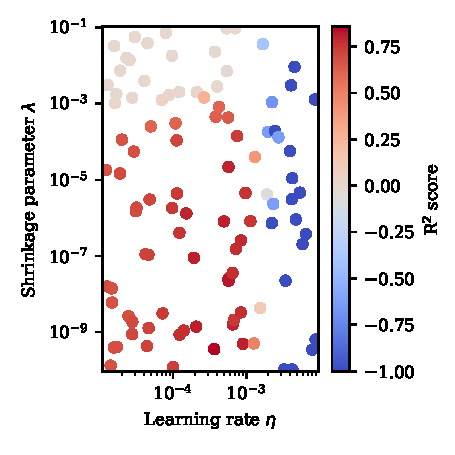
\includegraphics[scale=1]{{figures/nn_learning_rate_lambda_r2_franke_200_200_0.1}.pdf}
	\caption{$R^2$ score of validation set of Franke function data with 40 000 total points, $n_x=n_y=200,\ \sigma=0.1 $ using the multilayer perceptron regressor. The values of the shrinkage parameter $\lambda$ and the learning rate $\eta$ were chosen using randomized grid search.}
\end{figure}

\begin{figure*}
	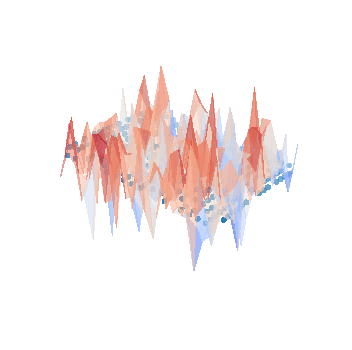
\includegraphics[width=\columnwidth]{{figures/3dplot_train_20_20_1.0}.pdf} 
	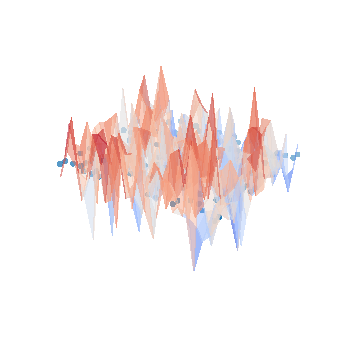
\includegraphics[width=\columnwidth]{{figures/3dplot_test_20_20_1.0}.pdf} 
	\caption{3D plot of the Franke function with added noise $\sim\mathcal{N}(0, \sigma^2)$ with $\sigma=1.0$. The dotted markers represent the regression model found using MLP. The left plot shows the model fitted on the training set, the right shows the model fitted on the test set. The total data set consist of 400 points, using two thirds $(\sfrac{2}{3})$ as the training set and the remaining points $(\sfrac{1}{3})$ as the test set. }
\end{figure*}

\begin{figure*}
	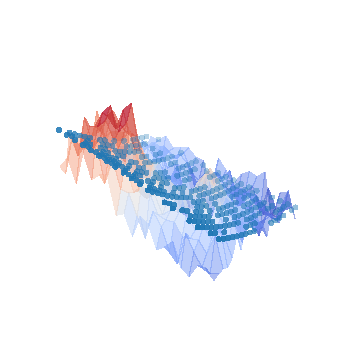
\includegraphics[width=\columnwidth]{{figures/3dplot_train_20_20_0.1}.pdf} 
	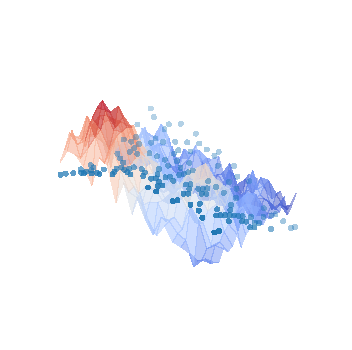
\includegraphics[width=\columnwidth]{{figures/3dplot_test_20_20_0.1}.pdf} 
	\caption{3D plot of the Franke function with added noise $\sim\mathcal{N}(0, \sigma^2)$ with $\sigma=0.1$. The dotted markers represent the regression model found using MLP. The left plot shows the model fitted on the training set, the right shows the model fitted on the test set. The total data set consist of 400 points, using two thirds $(\sfrac{2}{3})$ as the training set and the remaining points $(\sfrac{1}{3})$ as the test set. }
\end{figure*}

\begin{figure*}
	\includegraphics[width=\columnwidth]{{figures/3dplot_train_200_200_0.1}.pdf} 
	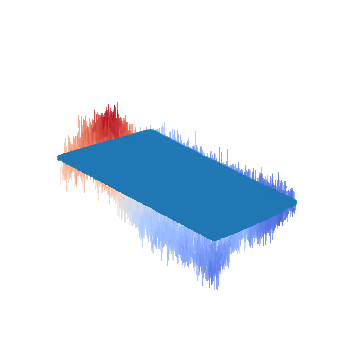
\includegraphics[width=\columnwidth]{{figures/3dplot_test_200_200_0.1}.pdf} 
	\caption{3D plot of the Franke function with added noise $\sim\mathcal{N}(0, \sigma^2)$ with $\sigma=0.1$. The dotted markers represent the regression model found using MLP. The left shows the model fitted on the training set, the right shows the model fitted on the test set. The total data set consist of 40 000 points, using two thirds $(\sfrac{2}{3})$ as the training set and the remaining points $(\sfrac{1}{3})$ as the test set. }
\end{figure*}

\section{Discussion}
fill
\section{Conclusion}
fill
\bibliographystyle{iEEEtran}
\bibliography{references}



\end{document}
